% -*- latex -*-
%%%%%%%%%%%%%%%%%%%%%%%%%%%%%%%%%%%%%%%%%%%%%%%%%%%%%%%%%%%%%%%%
%%%%%%%%%%%%%%%%%%%%%%%%%%%%%%%%%%%%%%%%%%%%%%%%%%%%%%%%%%%%%%%%
%%%%
%%%% This text file is part of the source of 
%%%% 'Parallel techniques'
%%%% by Ángel de Vicente, copyright 2019
%%%%
%%%% TO DO:
%%%%
%%%% intermediate-fortran.tex : intermediate fortran towards a
%%%%      Barnes-Hut N-body implementation
%%%% 
%%%%%%%%%%%%%%%%%%%%%%%%%%%%%%%%%%%%%%%%%%%%%%%%%%%%%%%%%%%%%%%%
%%%%%%%%%%%%%%%%%%%%%%%%%%%%%%%%%%%%%%%%%%%%%%%%%%%%%%%%%%%%%%%%

In order to implement the Barnes-Hut algorithm described in chapter
\ref{ch:barnes-hut.tex} we will need to learn some intermediate programming
concepts.

\Level 0 {Procedures and recursion}
\includepdf[frame=true,scale=0.98,pages={2-12,18-19}]{graphics/procedures_recursivity.pdf}

\Level 0 {Recursion exercises}
\label{sec:recursion-exercises}

You can find solutions to these exercises in section
\ref{app:sol-intermediate-fortran}, but you are \emph{highly encouraged} to try to solve
them first on your own.

A useful blog about recursion: \url{https://blog.angularindepth.com/learn-recursion-in-10-minutes-e3262ac08a1}


\Level 1 {Recursive Fibonacci function}
\label{ex:rec-fib}

Write a recursive function to calculate the Fibonacci numbers
\url{https://en.wikipedia.org/wiki/Fibonacci_number}

\Level 1 {Non-Recursive Fibonacci function}
\label{ex:nonrec-fib}

Write a non-recursive version of the function above and compare the execution
times of both versions for larger 'n' values (for example from 30-45). In Linux
you can check the execution time with the command 'time', for example:

\begin{verbatim}
time ./fibo_r 30
\end{verbatim}

\Level 1 {Memoized Recursive Fibonacci function}
\label{ex:memo_rec-fib}

Most probably, your recursive implementation is much slower than the iterative
version. Can you guess what is going on? [Modify the recursive routine to count
  the number of times that the fibonacci function is called. Then, look for
  information on "memoization" and try to modify the recursive routine so that
  you still use recursion, but in a way that it is as efficient as the iterative
  version. 

\Level 1 {Pseudo-code for printing a Binary Search Tree}
\label{ex:rec-bst}

Write pseudo-code, that is, without paying attention to the syntax of
 Fortran, a recursive function to print in ascending order a Binary Search Tree
 (\url{https://en.wikipedia.org/wiki/Binary_search_tree}). You can assume that your
 function will be given a tree estructure called "tree", and that these
 functions are provided to you: left\_branch\_exists(tree), which will return TRUE
 is "tree" has a left branch, right\_branch\_exists(tree), left\_branch(tree),
 which will return the left branch of the tree, right\_branch(tree), and
 node\_value(tree), which will return the value stored in the root node of the
 tree "tree".

\Level 1 {Tower of Hanoi game}
\label{ex:rec-hanoi}

Try to solve the Tower of Hanoi game \url{https://en.wikipedia.org/wiki/Tower_of_Hanoi}

 This is more difficult than the previous exercises, but it shows very nicely how
 useful recursion is in some cases. You assume that you have a pile of pieces
 (the code should work for any number of pieces) in column 1 and you want to
 move them to column 3. As for the previous exercise, start with just
 pseudo-code, so you can concentrate on the problem while forgetting about the
 details of Fortran. But this one is perfectly doable with the little Fortran we
 have learnt so far, so you could try to go for a full implementation.

 In the page \url{https://www.mathsisfun.com/games/towerofhanoi.html} you can see a
 demonstration of how to solve the puzzle and you can try to solve it by hand. A
 basic implementation to solve this problem is very easy, just needing a routine
 that prints the necessary movements to solve the puzzle (we do not need to
 store the state of the puzzle at all, only print the moves that would solve the
 game. When executing the code, we could just print the number of moves, where
 each move has the following format:

\begin{verbatim} 
 n (f -> t)
\end{verbatim} 

 where n is the piece number to move (1 is the smalles piece), f is the column
 whence the piece is coming, and t is the column where the piece is going
 to. For example:

\begin{verbatim} 
$ ./hanoi
 Enter number of pieces
3
           1 (           1  ->            3 )
           2 (           1  ->            2 )
           1 (           3  ->            2 )
           3 (           1  ->            3 )
           1 (           2  ->            1 )
           2 (           2  ->            3 )
           1 (           1  ->            3 )
\end{verbatim} 

\Level 1 {Recursive travelling salesman problem}
\label{ex:rec-tsp}

In section \ref{ex:basic-tsp} we looked at the Travelling Salesman Problem, but fixing it
 at 5 cities. Think about (and if possible implement) a recursive version that
 would work for any number of cities. If you understand how to write this one,
 then you are doing fantastic progress with recursion, as it gets a bit tricky
 to keep track of visited cities. If you don't get it at all, don't panic, we
 will see a solution in class.


\Level 1 {Contained digits}
\label{ex:rec-elf}

Write a recursive function that given two numbers: N1, N2, will say if all the
digits in N1 are contained in number N2.

For example, given (101,231001), we should return TRUE, since all digits in 101
are contained in 231001.

\Level 1 {Permutations of a number}
\label{ex:rec-perm}

Write a recursive subroutine that given a number N1, will print all possible
permutations of its digits. Assume for simplicity that N1 has no repeating
digits, and before you call the recursive subroutine place all the digits of N1
in an array. You can also use any other auxiliary arrays or scalars to keep
track of the permutations you have covered so far.

\Level 1 {8 queens problem}
\label{ex:rec-queens}

Try to find a way to solve the 8-queens puzzle (see
\url{https://en.wikipedia.org/wiki/Eight_queens_puzzle}). As always, start
without worrying about the implementation and just think about how you could
solve this problem (size = 8), assuming you could solve a smaller problem
(e.g. size = 7).

 
\Level 0 {Pointers and derived types}
{\includepdf[frame=true,scale=0.98,pages={2-21}]{graphics/pointers_derived_types.pdf}}

\Level 0 {Pointers exercises}
\label{sec:pointers-exercises}

You can find solutions to these exercises in section
\ref{app:sol-intermediate-fortran}, but you are \emph{highly encouraged} to try
to solve them first on your own.

\Level 1 {Pointer definitions}
\label{ex:pointer-def}

Specify two pointers, and let one of them point to a whole vector and the other
one point to the seventh element of the same vector. 


\Level 1 {Swapping numbers}
\label{ex:pointer-swap}

Write a subroutine that will use pointers as its arguments and will swap the
values of its two arguments. Write a main program that uses this function to
swap the values of two integer variables. Note: you will have to declare two
integer variables, plus two pointers to point to these variables and then make
the call to the subroutine which will be in charge of swapping the values of the
variables.


\Level 1 {Aliasing arrays}
\label{ex:pointer-alias-arrays}

Declare a one-dimensional array and two pointers, which you can use to assign
all even elements of a vector the value 13 and all odd elements of a vector the
value 17.  



\Level 0 {Pointers and recursion exercises}
\label{sec:pointers-recursion-exercises}

You can find solutions to these exercises in section
\ref{app:sol-intermediate-fortran}, but you are \emph{highly encouraged} to try
to solve them first on your own.


\Level 1 {Bi-directional list}
\label{ex:point-rec-bidirectional}

Modify the example ``Practical Example of Linked Lists'' in the slides, so that
the list will have links both to the previous and to the next element. Also
create a recursive subroutine that will print the list both forward and
backwards. You will have to take decisions, as to how many temporary pointers
you need, etc. You are free to do it in any way, as far as the list is properly
formed (i.e. it has links to the previous and next elements, and the ends of the
list are signalled with a pointer to NULL), and the routines for printing are
able to print the whole list forward and backwards.

\Level 1 {Sorted bi-directional list}
\label{ex:point-rec-sorted-bidirectional}

Modify exercise \ref{ex:point-rec-bidirectional} so that the elements are
inserted in the list sorted.

\Level 1 {Sort numbers with a Binary Search Tree}
\label{ex:point-rec-bst}

In this exercise we are going to build a binary search tree and then print the
tree (remember that we already solved with pseudo-code how to print a binary
search tree so that its elements will be printed sorted). The node structure is
basically the same as in exercise \ref{ex:point-rec-sorted-bidirectional}, but
now, instead of ``previous'' and ``next'', think of ``left'' and ``right''. So
first you will have to think of a procedure that will create the tree and then
another one to print the tree. Think carefully what you need, and above all make
sure that you never leave a node ``unattended'' (i.e. that you don't create
memory leaks by creating nodes and then deleting all pointers to it).

To make it easier, use this main code as a template, and just fill in the
routines ``place\_number'', and ``Print''. We don't want to deal with repeated
numbers, so if you give a repeated number, the procedure place\_number should
just ignore it and print a warning message.

\begin{verbatim}
PROGRAM listas
IMPLICIT NONE

TYPE CELL
INTEGER :: val
TYPE (CELL), POINTER :: left,right
END TYPE CELL

TYPE (CELL), POINTER :: head
INTEGER :: n,k,i

READ*, n

READ*, k
ALLOCATE(head)
head%val = k
NULLIFY(head%left)
NULLIFY(head%right)

DO i=2,n
READ*, k
CALL place_number(head,k)
END DO

CALL Print(head)

CONTAINS 
RECURSIVE SUBROUTINE place_number(node,number)
???
END SUBROUTINE place_number

RECURSIVE SUBROUTINE Print (node) 
???
END SUBROUTINE Print

END PROGRAM listas
\end{verbatim}

And remember to use input redirection so that you don't have to type in the
numbers everytime you run the code. For example, with the following
``numeros.txt'' file you could run the code as:

\begin{verbatim}
[angelv@nodo1]$ cat numbers.txt
10
6
3
15
2
7
2
5
4
21
31

[angelv@nodo1]$ ./tree < numbers.txt
INSERTING NUMBERS
-----------------
Repeated number 2, item ignored!

PRINTING BST
------------
2
3
4
5
6
7
15
21
31
[angelv@nodo1]$
\end{verbatim}

\Level 1 {Counting number of elements of a Binary Search Tree}
\label{ex:point-rec-nnodes-bst}
Add a function to the exercise \ref{ex:point-rec-bst}, that will return the
number of elements in a BST.

\Level 1 {Calculating the depth of a Binary Search Tree}
\label{ex:point-rec-depth-bst}
Add a function to the exercise \ref{ex:point-rec-bst}, that will return the
depth of a BST. An individual node would be depth=1, if this node has at least
one child node, then it would be depth=2, if it has ``grandchildren'', then it
would be depth=3, etc.

\Level 1 {Deleting a node in a Binary Search Tree -- DIFFICULT}
\label{ex:point-rec-delete-node-bst}

Add a function to the exercise \ref{ex:point-rec-bst}, that given a tree and a
number, it will delete the node with value==number (if it exists in the tree).

Before you try to code anything, you will have to make sure that you understand
the algorithm to delete the node, which you can check at
\url{https://en.wikipedia.org/wiki/Binary_search_tree#Deletion}


%% 7) (DIFÍCIL) Vamos a escribir una aplicación para buscar información
%% referente a viajes en avión y vamos a ver como usar arrays tradicionales no nos
%% servirá, debido a los grandes números a manejar. En el mundo hay aproximádamente
%% 18.000 aeropuertos comerciales
%% (http://www.aeronewstv.com/en/lifestyle/in-your-opinion/2954-how-many-commercial-airports-are-there-in-the-world.html)
%% y 5.000 aerolíneas (https://en.wikipedia.org/wiki/Lists_of_airlines). Si
%% quisiésemos representar todas las posibles combinaciones de vuelos entre las
%% distintas ciudades necesitaríamos un array de booleanos de tamaño
%% 18.000x18.000x5.000 (1.62e12), que ocuparía approx. 1.600 GB!
%% 
%% Como la mayoría de las combinaciones posibles simplemente no existirán, tenemos
%% que implementar algo parecido a una "sparse matrix", dónde solo almacenaremos
%% información sobre las combinaciones de vuelos que realmente existen. Como
%% ejemplo concreto, nuestro fichero de entrada podría ser:
%% 
%% 10 5000              ! 10 airports  5000 airlines
%% 2 10 4999 34.0       ! origin destination ariline price
%% 1 3 4002 5.0
%% 1 2 4003 4.0
%% 2 1 4010 34.0
%% 1 10 4010 200.0
%% 0 0 0 0
%% 
%% La primera línea nos indicará el número de aeropuertos (en este caso 10) y el
%% número de aerolíneas (en este caso 5000). El código tiene que poder funcionar
%% para cualquier número (razonable) de aeropuertos y compañías aereas. Las
%% siguientes líneas tienen cuatro números: id_origen id_destino id_aerolínea
%% precio. Esta información indica que existe un vuelo desde el aeropuerto
%% "id_origen" a "id_destino", volando con la compañía "id_aerolínea" y con un
%% coste de "precio". Una línea con todos los valores a 0 indica el final de los
%% datos.
%% 
%% Toda esta información la podemos almacenar en memoria como un array de
%% listas. Por ejemplo, para el fichero concreto de arriba, podríamos almacenarlo
%% como un array de tamaño el número de aeropuertos, donde cada elemento del array
%% apunta a una lista, donde cada elemento de la lista tiene la información sobre
%% cada conexión posible (i.e. aeropuerto de destino, aerolínea y precio).
%% 
%% ------
%% |  1 | [(3,4002,5.0),(2,4003,4.0),(10,4010,200.0)]
%% |  2 | [(10,4999,34.0),(1,4010,34.0)]
%% |  3 | []
%% |  4 | []
%% |  5 | []
%% |  6 | []
%% |  7 | []
%% |  8 | []
%% |  9 | []
%% | 10 | []
%% ------
%% 
%% Para construir esta estructura en Fortran, necesitaréis un array de punteros,
%% pero recordad que esto no se puede hacer en Fortran, así que necesitamos el
%% apaño de crear un tipo derivado (en este caso CPtr) cuyo único componente es un
%% puntero al tipo de datos que cada elemento de nuestra lista va a tener. Para
%% concretar, la parte de declaración de variables podría ser algo así:
%% 
%% ,----
%% | PROGRAM p1
%% |   IMPLICIT NONE
%% |   
%% |   TYPE nodo_con
%% |      INTEGER :: destination,airline
%% |      REAL    ::    price
%% |      TYPE(nodo_con), POINTER :: next
%% |   END type nodo_con
%% |   
%% |   TYPE CPtr
%% |      TYPE(nodo_con), POINTER :: nodo
%% |   END type CPtr
%% | 
%% |   TYPE(CPtr), ALLOCATABLE, DIMENSION(:) :: nodes
%% `----
%% 
%% Ahora vuestra tarea consiste en escribir el código para leer el fichero de
%% entrada, construir la estructura de datos representando los vuelos disponibles
%% y verificar que los datos se han almacenado correctamente. Además, querremos
%% implementar las siguientes funciones:
%% 
%% a) Generar para cada aerolínea la lista de todos sus vuelos (no imprimir
%% información para aerolíneas que no tengan ningún vuelo)
%% 
%% b) Dados un origen y un destino, ver si existe la posibilidad de viajar desde
%% origen a destino y decir el número de aviones (mínimo) que tendríamos que coger
%% para hacer el viaje.
%% 
%% c) Dado un origen y un precio máximo decir a todos los destinos que podríamos
%% viajar sin sobrepasar el presupuesto dado.
%% 
%% 
%% Como ejemplo de una ejecución posible (con las combinaciones de vuelos según lo
%% indicado arriba) de un código que implementa todas las funciones descritas
%% arriba podríamos tener:
%% 
%% ,----
%% | angelv@carro:~/Downloads$ ./p1 < p1.txt
%% |  BULDING GRAPH
%% |
%% |
%% |  
%% |  CHECKING GRAPH
%% |  Conexiones aeropuerto           1
%% |           10        4010   200.0000    
%% |            2        4003   4.000000    
%% |            3        4002   5.000000    
%% |  Conexiones aeropuerto           2
%% |            1        4010   34.00000    
%% |           10        4999   34.00000    
%% |  
%% |
%% |
%% |  CHECKING flights of all airlines
%% |  Connections for airline        4002
%% |            1           3        4002   5.000000    
%% |  Connections for airline        4003
%% |            1           2        4003   4.000000    
%% |  Connections for airline        4010
%% |            1          10        4010   200.0000    
%% |            2           1        4010   34.00000    
%% |  Connections for airline        4999
%% |            2          10        4999   34.00000    
%% |
%% |
%% |  
%% |  FINDING possible routes (enter A B, anyone 0 to end)
%% |  Checking possible route. Origin:           1 Destination:           3
%% |  Destination possible with number of hops:           1
%% |  
%% |  Checking possible route. Origin:           1 Destination:          10
%% |  Destination possible with number of hops:           1
%% |  
%% |  Checking possible route. Origin:           2 Destination:          10
%% |  Destination possible with number of hops:           1
%% |  
%% |  Checking possible route. Origin:           2 Destination:           3
%% |  Destination possible with number of hops:           2
%% |  
%% |  Checking possible route. Origin:           2 Destination:           4
%% |  Destination NOT POSSIBLE
%% |  
%% |
%% |  
%% |  FINDING possible cheap destinations (enter A price, any 0 to end)
%% |  Checking route. Origin:           1 Maximum price:   4.500000    
%% |  Destination:           2 for:   4.000000    
%% |  
%% |  Checking route. Origin:           1 Maximum price:   40.00000    
%% |  Destination:           2 for:   4.000000    
%% |  Destination:           3 for:   5.000000    
%% |  Destination:          10 for:   38.00000    
%% `----
%% \end{verbatim}


